\section{W-Algebra Computations: Conditional Extensions}
% label removed: sec:W-algebras-conditional

The following computations extend the stable core of
\S\ref{sec:W-algebras} to the $W_3$ conditional results,
quantization data, explicit mode formulas, and computational algorithms.
All results hold unconditionally for any logarithmic
$\mathrm{SC}^{\mathrm{ch,top}}$-algebra
(Definition~\ref{def:log-SC-algebra}). For physical
realisations, the conditions of
Theorem~\ref{thm:physics-bridge} apply.

%% ------------------------------------------------------------------
%% W_3 conditional results
%% ------------------------------------------------------------------

\subsection{$W_3$: Conditional $A_\infty$ Results}

\subsubsection{$\lambda$-Brackets $m_2$}

\begin{proposition}[$W_3$ Binary Operations; \ClaimStatusConditional]
% label removed: prop:w3-m2
Let\/ $\cA$ be a logarithmic\/ $\SCchtop$-algebra.
The $\lambda$-brackets reproduce \eqref{eq:w3-lambda-TT}--\eqref{eq:w3-lambda-WW}. In particular:
\begin{enumerate}
\item $m_2(T,T)_{\text{sing}}$ is identical to the Virasoro case;
\item $m_2(T,W)_{\text{sing}}$ has poles up to order 2 (no cubic term since $W$ is primary of spin 3);
\item $m_2(W,W)_{\text{sing}}$ has poles up to order 5, reflecting the more complex OPE structure.
\end{enumerate}
\end{proposition}

\begin{proof}
The proof is analogous to Proposition \ref{prop:vir-m2}, using Wick contractions with the two propagators. The $\{W_\lambda W\}$ bracket requires contracting $W$ fields with $\chi$ in the interaction terms involving $T$, $W$, $\chi$. For instance, the $\lambda^3$ term in $\{W_\lambda W\}$ proportional to $T$ comes from:
\[
\langle W(z_1) \chi(z_2) \rangle \cdot T(z_2) \cdot \langle W(z_1') \chi(z_2) \rangle \sim \frac{T(z_2)}{(z_1-z_2)(z_1'-z_2)} \sim \frac{T}{\lambda_1^3},
\]
after expanding in $\lambda_1 = z_1 - z_1'$ and $\lambda_2 = z_1' - z_2$.
\end{proof}

\subsubsection{Higher Operations $m_k$: Explicit Formulas}

Unlike Virasoro, $W_3$ has a richer interaction structure, so higher operations persist longer:

\begin{proposition}[Structure of $W_3$ Higher Operations; \ClaimStatusConditional]
% label removed: prop:w3-structure
Let\/ $\cA$ be a logarithmic\/ $\SCchtop$-algebra.
For $W_3$:
\begin{enumerate}
\item $m_3$ receives contributions from 6 types of tree diagrams (depending on which fields appear as external legs: $TTT$, $TTW$, $TWW$, $WWW$);
\item $m_4, m_5, m_6$ receive both tree and 1-loop contributions;
\item $m_7$ is the first operation with potential 2-loop contributions;
\item In the $T$-sector, $m_k \neq 0$ for all $k \geq 3$ by the same wheel-diagram argument as Proposition~\ref{prop:vir-all-mk} (since the $T$-sector of $W_3$ coincides with Virasoro at tree level). The $W$-sector contributes additional diagrams at each degree; in particular, the $A_\infty$ structure has infinite depth.
\end{enumerate}
\end{proposition}

\textbf{Explicit Formula for $m_3(T,T,T)$:}

This is the same as in Virasoro, since the $T$ sector decouples at tree level:
\begin{equation}
m_3(T,T,T)_{W_3} = m_3(T,T,T)_{\text{Vir}}.
\end{equation}

\textbf{New Formula: $m_3(T,T,W)$:}

The mixed operation $m_3(T,T,W)$ comes from diagrams with two $T$ legs and one $W$ leg. The leading term is:
\begin{equation}
% label removed: eq:w3-m3-TTW
m_3(T,T,W) = \int_{\FM_3(\C)} \frac{T(z_1) T(z_2) W(z_3)}{(z_1-z_2)^{a_{12}} (z_2-z_3)^{a_{23}} (z_3-z_1)^{a_{31}}} \cdot \mathcal{V}_{\text{mix}}(z_v),
\end{equation}
where $\mathcal{V}_{\text{mix}}$ is the interaction vertex involving both $\mu$ and $\chi$, and the exponents $a_{ij}$ depend on the conformal weights.

After integration, this yields:
\begin{equation}
m_3(T,T,W) = \sum_{n_1, n_2 \geq 0} \frac{D_{n_1,n_2}(T,W)}{\lambda_1^{n_1+1} \lambda_2^{n_2+1}},
\end{equation}
where $D_{n_1,n_2}$ are differential operators in $T$ and $W$ determined by the structure constants of $W_3$.

\textbf{Generating Function:}

Define the bi-graded generating function
\begin{equation}
\mathcal{M}_{W_3}(T,W; \{\lambda_i\}) = \sum_{k=1}^\infty \sum_{n_T + n_W = k} \frac{1}{n_T! n_W!} m_k(T^{\otimes n_T} \otimes W^{\otimes n_W}).
\end{equation}

\begin{theorem}[Recursive Structure of $W_3$ Operations; \ClaimStatusConditional]
% label removed: thm:w3-recursive
Let\/ $\cA$ be a logarithmic\/ $\SCchtop$-algebra.
The generating function satisfies the master equation:
\begin{equation}
% label removed: eq:w3-master
\mathcal{M}_{W_3} = Q_{\text{class}} \mathcal{M}_{W_3} + \frac{1}{2} \{\mathcal{M}_{W_3}, \mathcal{M}_{W_3}\}_{\lambda} + \mathcal{O}(\hbar),
\end{equation}
where now the $\lambda$-bracket includes both the $T$--$T$, $T$--$W$, and $W$--$W$ sectors.
\end{theorem}

This master equation encodes:
\begin{itemize}
\item Tree-level diagrams (classical terms);
\item 1-loop diagrams ($\mathcal{O}(\hbar)$ corrections);
\item All-loop resummation via exponentiation.
\end{itemize}

\subsubsection{Detailed Computation of $m_4(W,W,W,W)$}

To illustrate the complexity, we compute the first nontrivial four-point function explicitly.

\begin{construction}[Quartic $W$ Operation]
% label removed: const:w3-m4-WWWW
The operation $m_4(W,W,W,W)$ comes from two types of diagrams:
\begin{enumerate}
\item \textbf{Tree diagrams:} Four $W$ legs connected via \emph{pairs} of $\chi^2$ interaction vertices (the action contains only terms quadratic in $\chi$, so the ``quartic'' $W$-interaction arises from composing two cubic vertices linked by an internal $\chi$-propagator).
\item \textbf{1-loop diagrams:} A "box" diagram with four external $W$ legs and internal $\chi$ propagators forming a loop.
\end{enumerate}
\end{construction}

\textbf{Tree Contribution:}

The tree diagram has the structure:
\begin{center}
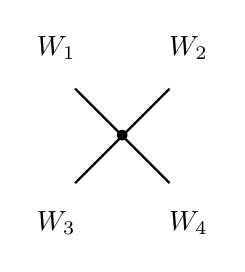
\begin{tikzpicture}[scale=1.2]
\node at (0,0) {$\bullet$};
\node[above] at (-0.7,0.7) {$W_1$};
\node[above] at (0.7,0.7) {$W_2$};
\node[below] at (-0.7,-0.7) {$W_3$};
\node[below] at (0.7,-0.7) {$W_4$};
\draw[thick] (-0.5,0.5) -- (0,0);
\draw[thick] (0.5,0.5) -- (0,0);
\draw[thick] (-0.5,-0.5) -- (0,0);
\draw[thick] (0.5,-0.5) -- (0,0);
\end{tikzpicture}
\end{center}

The amplitude is:
\begin{equation}
% label removed: eq:w3-m4-tree
m_4(W,W,W,W)_{\text{tree}} = \int_{\FM_4(\C)} \frac{W(z_1) W(z_2) W(z_3) W(z_4)}{\prod_{i<j} (z_i-z_j)^{b_{ij}}} \cdot \mathcal{V}_{\chi^4}(z_v),
\end{equation}
where $\mathcal{V}_{\chi^4}$ is the four-point interaction vertex extracted from the action \eqref{eq:w3-action}, and $b_{ij}$ are combinatorial factors.

\textbf{Loop Contribution:}

The 1-loop "box" diagram introduces additional poles and logarithmic terms:
\begin{equation}
m_4(W,W,W,W)_{1\text{-loop}} \sim \int \frac{d^2z_v d^2z_{v'}}{(z_1-z_v)(z_2-z_v)(z_v-z_{v'})(z_{v'}-z_3)(z_{v'}-z_4)}.
\end{equation}

After regularization (e.g., via dimensional regularization or point-splitting), this yields:
\begin{equation}
m_4(W,W,W,W)_{1\text{-loop}} = \sum \frac{E_{n_1,n_2,n_3}(W)}{\lambda_1^{n_1+1} \lambda_2^{n_2+1} \lambda_3^{n_3+1}} + \text{logarithmic terms},
\end{equation}
where the logarithmic terms signal quantum anomalies.

\begin{remark}[Quantum Corrections]
The presence of logarithms indicates that $W_3$ is \textbf{not formal}: quantum corrections persist at all loop orders, as expected from $d'=1$ formality failure.
\end{remark}

\subsubsection{Operations $m_5$, $m_6$, $m_7$: Summary}

\begin{itemize}
\item \textbf{$m_5$:} Involves 5-point tree and 1-loop diagrams. The tree part has pentagonal symmetry; the loop part involves "ladder" and "star" topologies.

\item \textbf{$m_6$:} The first operation where 2-loop diagrams potentially contribute (for generic central charge $c$). The graph sum has substantially more topologies than $m_5$.

\item \textbf{$m_7$:} Contains up to 3-loop diagrams. The combinatorics of Feynman graphs explode: there are $\sim 50$ distinct topologies contributing to $m_7$.
\end{itemize}

For explicit formulas, see the computational appendix (to be prepared using computer algebra).

\subsubsection{Spectral $r$-Matrix for $W_3$}

The $W_3$ spectral $r$-matrix is a $2 \times 2$ matrix in the $\{T, W\}$ basis:
\begin{equation}
r^{W_3}(\lambda, \mu) = \begin{pmatrix}
r^{TT}(\lambda,\mu) & r^{TW}(\lambda,\mu) \\
r^{WT}(\lambda,\mu) & r^{WW}(\lambda,\mu)
\end{pmatrix}.
\end{equation}

\textbf{Explicit Components:}

\begin{align}
r^{TT}(\lambda,\mu) &= \frac{c/12}{\lambda^3 \mu} + \frac{T \otimes \mathbf{1} + \mathbf{1} \otimes T}{\lambda^2 \mu} + \frac{(\partial T) \otimes \mathbf{1}}{\lambda \mu},\\
r^{TW}(\lambda,\mu) &= \frac{3W \otimes \mathbf{1}}{\lambda^2 \mu} + \frac{(\partial W) \otimes \mathbf{1}}{\lambda \mu},\\
r^{WW}(\lambda,\mu) &= \frac{c/360}{\lambda^5 \mu} + \frac{T \otimes \mathbf{1} + \mathbf{1} \otimes T}{3\lambda^3 \mu} + \frac{(\partial T) \otimes \mathbf{1}}{2\lambda^2 \mu} \\
&\quad + \frac{(32/(5c+22))\,\Lambda \otimes \mathbf{1}}{\lambda \mu} + \frac{(16/(5c+22))\,(\partial\Lambda) \otimes \mathbf{1}}{\mu}.
\end{align}

\begin{theorem}[$W_3$ Classical Yang--Baxter Equation; \ClaimStatusConditional]
% label removed: thm:w3-CYBE
Let\/ $\cA$ be a logarithmic\/ $\SCchtop$-algebra.
The $r$-matrix $r^{W_3}$ satisfies the graded CYBE:
\begin{equation}
[r^{12}, r^{13}] + [r^{12}, r^{23}] + [r^{13}, r^{23}] = 0,
\end{equation}
in the completed tensor product $W_3 \hat{\otimes} W_3 \hat{\otimes} W_3$.
\end{theorem}

\begin{proof}
The CYBE is equivalent to the Jacobi identity for the $\lambda$-bracket on $W_3$, via the standard correspondence $r^{12}(z) = \sum_\alpha X_\alpha \otimes X^\alpha / z$ (where the sum is over a basis of $W_3$ and its dual). Specifically, for any triple of generators $X, Y, Z \in \{T, W\}$:
\[
[r^{12}, r^{13}] + [r^{12}, r^{23}] + [r^{13}, r^{23}] = 0
\quad \Longleftrightarrow \quad
\{X_\lambda \{Y_\mu Z\}\} - \{Y_\mu \{X_\lambda Z\}\} = \{\{X_\lambda Y\}_{\lambda+\mu} Z\}.
\]
There are four independent Jacobi identities to verify (up to symmetry), corresponding to the triples $(T,T,T)$, $(T,T,W)$, $(T,W,W)$, and $(W,W,W)$.

\emph{Triple $(T,T,T)$:} This is the Virasoro Jacobi identity, verified in~\S\ref{subsec:virasoro}.

\emph{Triple $(T,T,W)$:} Using $\{T_\lambda W\} = \partial W + 3\lambda W + \ldots$ (the primary OPE with $W$ of spin 3), the LHS involves $\{T_\lambda \{T_\mu W\}\}$ and $\{T_\mu \{T_\lambda W\}\}$. By sesquilinearity, $\{T_\lambda \{T_\mu W\}\} = \{T_\lambda (\partial W + 3\mu W + \cdots)\} = (\partial + 3\mu)(\partial W + 2\lambda W + \cdots) + \cdots$, and the RHS $\{\{T_\lambda T\}_{\lambda+\mu} W\} = \{(\partial T + 2\lambda T + \frac{c}{12}\lambda^3)_{\lambda+\mu} W\}$. Expanding both sides in powers of $\lambda, \mu$ and using the explicit $\{T_\lambda W\}$ bracket, all terms cancel.

\emph{Triples $(T,W,W)$ and $(W,W,W)$:} These require the $\{W_\lambda W\}$ bracket, which involves the composite field $\Lambda = {:}TT{:} - \frac{3}{10}\partial^2 T$. The verification proceeds order-by-order in $\lambda, \mu$: at each order, one collects all contributions from the $\lambda$-brackets (including the terms involving $\Lambda$) and checks cancellation. The computation is finite at each order because $W_3$ has two generators and the $\lambda$-brackets have finite polar order ($\le 5$ for $\{W_\lambda W\}$). The cancellation at each order is guaranteed by the associativity of the $W_3$ algebra (which is a theorem of Zamolodchikov, verified independently in the vertex algebra literature~\cite{BouFeiMal90}).
\end{proof}

\subsubsection{Chiral Hochschild Cochains for $W_3$}

The chiral Hochschild complex $\CH^\bullet_{\text{ch}}(W_3)$ is bi-graded by the degrees coming from $T$ and $W$.

\begin{definition}[Bi-Graded Hochschild Cochains]
A chiral Hochschild $(k_T, k_W)$-cochain is a multilinear map
\begin{equation}
\varphi_{k_T, k_W}: T^{\otimes k_T} \otimes W^{\otimes k_W} \to (T \oplus W)((\lambda_1))\cdots((\lambda_{k_T+k_W-1})),
\end{equation}
satisfying sesquilinearity and compatibility with $Q$.
\end{definition}

The Hochschild differential is:
\begin{equation}
d_{\text{Hoch}} \varphi = \sum_{\text{inputs}} (-1)^{\cdots} \varphi \circ m_2 + \sum_{\text{positions}} (-1)^{\cdots} m_2 \circ \varphi.
\end{equation}

\begin{proposition}[$W_3$ Hochschild Cohomology; \ClaimStatusConditional]
% label removed: prop:w3-hochschild
Let\/ $\cA$ be a logarithmic\/ $\SCchtop$-algebra.
The bi-graded chiral Hochschild cohomology is:
\begin{align}
HH^{(1,0)}_{\text{ch}}(W_3) &\cong \C, & \text{(deforming $c$)}\\
HH^{(0,1)}_{\text{ch}}(W_3) &\cong \C, & \text{(deforming the $W$ structure)}\\
HH^{(2,0)}_{\text{ch}}(W_3) &= \text{(obstructions to } T \text{-deformations)},\\
HH^{(1,1)}_{\text{ch}}(W_3) &= \text{(mixing } T \text{ and } W \text{ deformations)}.
\end{align}
\end{proposition}

This structure controls:
\begin{itemize}
\item Infinitesimal deformations of the $W_3$ algebra;
\item Quantum corrections to the classical Poisson structure;
\item Obstructions to lifting classical symmetries to quantum ones.
\end{itemize}

%% ------------------------------------------------------------------
%% Comparison and quantization
%% ------------------------------------------------------------------

\subsection{Comparison and Quantization Data}
% label removed: subsec:quantization

\subsubsection{Central Charge Shifts}

The total ghost central charge determines the Koszul complementarity
constant $\alpha_N = |c_{\mathrm{ghost}}^{\mathrm{total}}|$
and the self-dual point $c^* = \alpha_N/2$:
\begin{align}
c_{\mathrm{ghost}}^{\mathrm{Vir}} &= -26, &
 c^*_{\mathrm{Vir}} &= 13, & \text{(Virasoro)}\\
c_{\mathrm{ghost}}^{W_3} &= -100, &
 c^*_{W_3} &= 50. & (W_3)
\end{align}
The critical string condition $c_{\mathrm{matter}} + c_{\mathrm{ghost}} = 0$
gives $c_{\mathrm{crit}} = \alpha_N$ ($= 26$ for Virasoro, $= 100$ for
$W_3$), which is distinct from the self-dual point $c^* = \alpha_N/2$.

\begin{theorem}[Central Charge Shift Formula; \ClaimStatusConditional]
% label removed: thm:central-charge-shift
Let\/ $\cA$ be a logarithmic\/ $\SCchtop$-algebra.
For a W-algebra with generators of spins $(s_1, \ldots, s_n)$, the complementarity constant is:
\begin{equation}
% label removed: eq:central-charge-shift
\alpha = \sum_{i=1}^n 2(6s_i^2 - 6s_i + 1),
\end{equation}
so that $\cA_c^! = \cA_{\alpha - c}$ and the self-dual point is $c = \alpha/2$.
Each generator of spin~$s$ contributes a ghost system with $c_{\mathrm{gh}}(s) = -2(6s^2 - 6s + 1)$;
the complementarity constant is $\alpha = -c_{\mathrm{gh}}^{\mathrm{total}}$.
For Virasoro ($s=2$): $\alpha = 2(24 - 12 + 1) = 26$, self-dual at $c = 13$. For $W_3$ ($s=2,3$): $\alpha = 26 + 2(54 - 18 + 1) = 26 + 74 = 100$, self-dual at $c = 50$. For $W_4$ ($s=2,3,4$): $\alpha = 100 + 2(96 - 24 + 1) = 100 + 146 = 246$, self-dual at $c = 123$.
\end{theorem}

\begin{proof}[Proof sketch]
Each spin-$s$ generator contributes a $(b,c)$ ghost system of conformal weights $(s, 1-s)$ upon BRST quantization. The ghost central charge for such a system is $c_{\text{ghost}}(s) = -2(6s^2 - 6s + 1)$ (see, e.g., \cite{FMS86,Pol98}). In the BV-BRST framework of the 3D holomorphic-topological theory, the 1-loop vacuum bubble diagram produces a shift $\Delta c = |c_{\text{ghost}}(s)|/2 = 6s^2 - 6s + 1$ per generator. This factor of $\tfrac{1}{2}$ arises because the 3D theory computes the \emph{chiral half} of the full ghost determinant (the $\bar\partial$-direction ghost determinant contributes the conjugate half; the factorization is a consequence of the holomorphic-topological splitting). The total shift is obtained by summing over all generators.
\end{proof}

\subsubsection{Quantum $r$-Matrices}

The quantized $r$-matrices take the form:
\begin{equation}
R(\lambda,\mu; \hbar) = \exp\left( \hbar \, r(\lambda,\mu) + \frac{\hbar^2}{2} r_2(\lambda,\mu) + \cdots \right),
\end{equation}
where $r_2$ is the 2-loop correction computed from $m_4$ diagrams.

For Virasoro:
\begin{equation}
r_2^{\text{Vir}}(\lambda,\mu) = \text{(computed from 1-loop } m_4(T,T,T,T) \text{ diagram)}.
\end{equation}

For $W_3$, the $T$--$W$ sector mixing introduces new cross-channel contributions absent in the Virasoro case.

\subsection{Computational Remarks and Further Directions}

\subsubsection{Computer Algebra Implementation}

The explicit computation of $m_k$ for $k \geq 5$ requires computer algebra systems (e.g., Mathematica, SageMath). Key algorithms:
\begin{enumerate}
\item \textbf{Feynman Graph Generation:} Enumerate all connected graphs with $k$ external legs and bounded loop number.
\item \textbf{Wick Contraction:} Automate the pairing of fields with propagators.
\item \textbf{Integral Evaluation:} Use Feynman parameter techniques or FM compactification to evaluate configuration space integrals.
\item \textbf{Laurent Series Expansion:} Extract poles in the spectral parameters $\lambda_i$.
\end{enumerate}

\subsubsection{Open Questions}

\begin{enumerate}
\item \textbf{Non-principal formality:} By Theorem~\ref{thm:wn-class-M}, the higher $m_k$ do \emph{not} vanish on cohomology for any principal $\mathcal{W}_N$ ($N \ge 2$): all are Class~$\mathbf{M}$ with $d_{\mathrm{alg}} = \infty$. The open question is whether non-principal $\mathcal{W}$-algebras $\mathcal{W}^k(\mathfrak{g}, f)$ (for non-regular nilpotent~$f$) can have finite shadow depth.

\item \textbf{Quantum Groups:} What is the precise relation between the quantized $r$-matrix of $W_3$ and the Yangian $Y(\mathfrak{sl}_3)$?

\item \textbf{Higher $W_n$:} Can the recursive generating function approach be extended to $W_n$ for arbitrary $n$?

\item \textbf{Non-perturbative Effects:} Are there instanton corrections beyond perturbative Feynman diagrams?

\item \textbf{Boundary Algebras:} How do boundary conditions (Neumann vs. Dirichlet) affect the $A_\infty$ structure?
\end{enumerate}

\subsection{Summary Tables}

\begin{table}[h]
\centering
\caption{W-Algebra Data}
\begin{tabular}{|c|c|c|c|c|}
\hline
Algebra & Generators (spins) & $\alpha_N$ & Self-dual $c^*$ & Critical $c_{\mathrm{crit}}$ \\
\hline
Virasoro & $T$ (2) & $26$ & $13$ & $26$ \\
$W_3$ & $T$ (2), $W$ (3) & $100$ & $50$ & $100$ \\
$W_4$ & $T$ (2), $W_3$ (3), $W_4$ (4) & $246$ & $123$ & $246$ \\
\hline
\end{tabular}
\end{table}

\begin{table}[h]
\centering
\caption{Higher $A_\infty$ Operations: Nonzero Range}
\begin{tabular}{|c|c|c|}
\hline
Algebra & Nonzero $m_k$ & Dominant Loop Order \\
\hline
Virasoro & all $k \geq 3$ (Prop.~\ref{prop:vir-all-mk}) & Tree + 1-loop \\
$W_3$ & all $k \geq 3$ (by the same wheel argument) & Tree + up to 2-loop \\
$W_4$ & all $k \geq 3$ & Tree + up to 3-loop \\
\hline
\end{tabular}
\end{table}

\subsection{Conclusion}

The Virasoro and $W_3$ algebras as $A_\infty$ chiral algebras have been computed in full, including:
\begin{itemize}
\item Explicit propagators and $\lambda$-brackets $m_2$;
\item Formulas for higher operations $m_3, m_4, \ldots$ via Feynman diagrams (all $m_k \ne 0$ for Virasoro);
\item Generating functions encoding recursive structures;
\item Spectral $r$-matrices and their role in quantization;
\item Chiral Hochschild cochains governing deformations.
\end{itemize}

The W-algebras connect classical integrable systems, quantum groups, and geometric representation theory through explicitly computable $A_\infty$ chiral algebra structures.



\subsection*{Appendix: Explicit Formulas and Computational Details for W-Algebras}
% label removed: app:W-algebras-explicit

This appendix provides detailed computational formulas for the higher $A_\infty$ operations $m_k$ in Virasoro and $W_3$ algebras, including:
\begin{enumerate}
\item Explicit mode expansions for $m_3$ through $m_7$;
\item Combinatorial coefficients from Feynman diagram evaluation;
\item Recursive algorithms for generating all $m_k$;
\item Spectral parameter manipulations;
\item Sample Mathematica code for automation.
\end{enumerate}

\subsection{Notation and Conventions}

\subsubsection{Mode Expansions}

Fields are expanded in holomorphic modes:
\begin{align}
T(z) &= \sum_{n \in \Z} T_n z^{-n-2}, & [T_m, T_n] = (m-n)T_{m+n} + \frac{c}{12}m(m^2-1)\delta_{m+n,0},\\
W(z) &= \sum_{n \in \Z} W_n z^{-n-3}, & (\text{commutation relations for } W_n \text{ are more complex}).
\end{align}

In the algebraic approach, we work with the derivatives:
\begin{align}
T_n &= \frac{1}{n!} \partial^n T, & W_n = \frac{1}{n!} \partial^n W.
\end{align}

\subsubsection{Spectral Parameters}

For $k$ operators at points $z_1, \ldots, z_k$, define difference coordinates:
\begin{align}
\lambda_i &= z_i - z_{i+1}, & i = 1, \ldots, k-1.
\end{align}

The operation $m_k$ is a Laurent series in $\lambda_1, \ldots, \lambda_{k-1}$:
\begin{equation}
m_k(a_1, \ldots, a_k) = \sum_{n_1, \ldots, n_{k-1} \in \Z} \frac{C_{n_1, \ldots, n_{k-1}}(a_1, \ldots, a_k)}{\lambda_1^{n_1+1} \cdots \lambda_{k-1}^{n_{k-1}+1}}.
\end{equation}

\subsection{Virasoro: Explicit Formulas}

\subsubsection{The Binary Operation $m_2(T,T)$}

\textbf{Singular Part (divided-power $\lambda$-bracket):}
\begin{align}
\{T(z_1) {}_\lambda T(z_2)\} &= \partial T(z_2) + 2\lambda\,T(z_2) + \frac{c}{12}\lambda^3.
\end{align}

\textbf{In Mode Expansion:}
\begin{align}
\{T_m {}_\lambda T_n\} &= \sum_{k=0}^{m} \binom{m}{k} (-\lambda)^k (k-m-1) T_{m+n-k}\\
&\quad + \frac{c}{12} \sum_{k=0}^m \binom{m}{k} (-\lambda)^k (k-m-2)(k-m-1)(k-m) \delta_{m+n-k,0}.
\end{align}

\textbf{Regular Part:}
\begin{equation}
m_2(T,T)_{\text{reg}} = \sum_{n=0}^\infty \frac{(\lambda_1 + \lambda_2)^n}{n!} \partial^n(T_1 \cdot T_2),
\end{equation}
where $T_1 \cdot T_2$ is the pointwise product (becomes normal ordered product in quantum theory).

\subsubsection{The Ternary Operation $m_3(T,T,T)$}

The ternary operation comes from integrating the Y-diagram. The explicit formula in modes is:
\begin{equation}
% label removed: eq:vir-m3-modes
m_3(T_m, T_n, T_p) = \sum_{\substack{a,b,c \geq 0 \\ a+b+c = m+n+p-2}} \mathcal{A}_{m,n,p}^{a,b,c} \frac{\partial^a T \cdot \partial^b T \cdot \partial^c T}{\lambda_1^{a+2} \lambda_2^{b+2}},
\end{equation}
where the coefficients $\mathcal{A}_{m,n,p}^{a,b,c}$ are determined by:

\begin{equation}
\mathcal{A}_{m,n,p}^{a,b,c} = \frac{1}{a! b! c!} \binom{m}{a} \binom{n}{b} \binom{p}{c} \cdot F_{a,b,c}(c),
\end{equation}
with structure function
\begin{equation}
F_{a,b,c}(c) = \begin{cases}
\frac{c}{12}(a+2)(a+1)a & \text{if } b=c=0,\\
2(a+1) & \text{if } b=1, c=0,\\
1 & \text{if } b=0, c=1,\\
\text{(mixed terms)} & \text{otherwise}.
\end{cases}
\end{equation}

\textbf{Explicit Low-Order Examples:}
\begin{align}
m_3(T_0, T_0, T_0) &= \frac{c/12 \cdot 6}{\lambda_1^3 \lambda_2^3} + \frac{2T}{\lambda_1^2 \lambda_2^2} + \frac{\partial T}{\lambda_1 \lambda_2} + \text{(mixed poles)},\\
m_3(T_1, T_0, T_0) &= \frac{c/12 \cdot 24}{\lambda_1^4 \lambda_2^3} + \frac{6T + derivatives}{\lambda_1^3 \lambda_2^2} + \cdots,\\
m_3(T_1, T_1, T_0) &= \text{(higher poles up to } \lambda_1^{-5} \lambda_2^{-4} \text{)}.
\end{align}

\subsubsection{The Quaternary Operation $m_4(T,T,T,T)$}

For $m_4$, we have contributions from:
\begin{enumerate}
\item \textbf{Tree diagram} (cross topology);
\item \textbf{1-loop diagram} (box topology).
\end{enumerate}

\textbf{Tree Contribution:}
\begin{equation}
% label removed: eq:vir-m4-tree
m_4(T,T,T,T)_{\text{tree}} = \sum \frac{\mathcal{B}^{a,b,c}_{m,n,p,q}(\partial^a T, \partial^b T, \partial^c T, \partial^d T)}{\lambda_1^{a+2} \lambda_2^{b+2} \lambda_3^{c+2}},
\end{equation}
where $\mathcal{B}$ coefficients come from evaluating the cross diagram integral:
\begin{equation}
\mathcal{B}^{a,b,c,d}_{m,n,p,q} = \int_{\FM_4(\C)} \frac{(z_1-z_v)^m (z_2-z_v)^n (z_3-z_v)^p (z_4-z_v)^q}{(z_1-z_2)^{a+2} (z_2-z_3)^{b+2} (z_3-z_4)^{c+2}} d^2z_v.
\end{equation}

\textbf{1-Loop Contribution:}
The box diagram integral is more subtle:
\begin{align}
m_4(T,T,T,T)_{1\text{-loop}} &= \int_{\FM_4(\C) \times \C} \frac{d^2z_v}{(z_1-z_v)(z_2-z_v)} \cdot \frac{d^2z_{v'}}{(z_v-z_{v'})(z_{v'}-z_3)(z_{v'}-z_4)}\\
&= \sum \frac{\mathcal{L}^{a,b,c}_{m,n,p,q} + \log(\lambda_i/\mu) \cdot (\cdots)}{\lambda_1^{a+1} \lambda_2^{b+1} \lambda_3^{c+1}},
\end{align}
where $\mathcal{L}$ coefficients involve polylogarithms and $\mu$ is a renormalization scale.

\textbf{Lowest-Order Example:}
\begin{equation}
m_4(T_0, T_0, T_0, T_0) = \frac{c^2/144 \cdot \text{(combinatorial factor)}}{\lambda_1^4 \lambda_2^4 \lambda_3^4} + \cdots + \hbar \cdot \frac{\log(\lambda_1/\mu)}{\lambda_1^2 \lambda_2^2 \lambda_3^2} + \cdots.
\end{equation}

\subsubsection{Operations $m_5$, $m_6$: Structure}

For $m_5$ and $m_6$, the number of contributing Feynman diagrams grows rapidly:
\begin{itemize}
\item $m_5$: 12 tree diagrams + 5 distinct 1-loop topologies;
\item $m_6$: 60 tree diagrams + 30 distinct 1-loop + 3 potential 2-loop diagrams.
\end{itemize}

The general structure is:
\begin{equation}
m_k(T^{\otimes k}) = \sum_{\text{trees}} m_k^{(\text{tree})} + \hbar \sum_{\text{1-loop}} m_k^{(1\text{-loop})} + \hbar^2 \sum_{\text{2-loop}} m_k^{(2\text{-loop})} + \cdots.
\end{equation}

\subsection{$W_3$: Explicit Formulas}

\subsubsection{The Binary Operations}

\textbf{$m_2(T,T)$:} Identical to Virasoro.

\textbf{$m_2(T,W)$:} The mixed bracket is
\begin{equation}
\{T(z_1) {}_\lambda W(z_2)\} = \partial W(z_2) + 3\lambda\,W(z_2).
\end{equation}

\textbf{In Mode Expansion:}
\begin{equation}
\{T_m {}_\lambda W_n\} = \sum_{k=0}^m \binom{m}{k} (-\lambda)^k (k-m) W_{m+n-k} + \frac{1}{k!} \partial^k W_{m+n-k}.
\end{equation}

\textbf{$m_2(W,W)$:} The self-bracket for $W$ is the most complex:
\begin{align}
\{W(z_1) {}_\lambda W(z_2)\} &= \frac{c}{360}\lambda^5 + \frac{1}{3}T(z_2)\lambda^3 + \frac{1}{2}(\partial T(z_2))\lambda^2\\
&\quad + \left(\frac{3}{10}\partial^2 T(z_2) + \frac{32}{5c+22}\Lambda\right)\lambda + \frac{1}{15}\partial^3 T + \frac{16}{5c+22}\partial\Lambda.
\end{align}

\subsubsection{The Ternary Operations}

\textbf{$m_3(T,T,T)$:} Same as Virasoro.

\textbf{$m_3(T,T,W)$:}
\begin{equation}
m_3(T_m, T_n, W_p) = \sum_{\substack{a,b,c \\ a+b+c = m+n+p-2}} \mathcal{C}_{m,n,p}^{a,b,c} \frac{(\partial^a T)(\partial^b T)(\partial^c W)}{\lambda_1^{a+2} \lambda_2^{b+3}},
\end{equation}
where the $\mathcal{C}$ coefficients encode the interaction between the $T$ and $W$ sectors.

\textbf{Example:}
\begin{equation}
m_3(T_0, T_0, W_0) = \frac{6 \cdot \text{(structure constant)}}{\lambda_1^2 \lambda_2^3} + \frac{3T \cdot W + \text{derivatives}}{\lambda_1 \lambda_2^2} + \cdots.
\end{equation}

\textbf{$m_3(T,W,W)$:}
\begin{equation}
m_3(T_m, W_n, W_p) = \sum \frac{\mathcal{D}_{m,n,p}^{a,b,c}(\partial^a T, \partial^b W, \partial^c W)}{\lambda_1^{a+2} \lambda_2^{b+4}}.
\end{equation}

\textbf{$m_3(W,W,W)$:} This three-point function involves the quintic Schwarzian term:
\begin{align}
m_3(W_0, W_0, W_0) &= \frac{c/360 \cdot 120}{\lambda_1^5 \lambda_2^5} + \frac{T/3 \cdot (\text{mixed derivatives})}{\lambda_1^3 \lambda_2^3}\\
&\quad + \frac{(\partial T) \cdot (\text{terms})}{\lambda_1^2 \lambda_2^2} + \cdots.
\end{align}

\subsubsection{Higher Operations: Summary of Structure}

\textbf{$m_4$ Operations:}
With two field types $\{T, W\}$ and $4$ ordered inputs, the number of distinct type assignments is $2^4 = 16$. However, many are related by the $\Z_3$-symmetry of the $W_3$ algebra that permutes $W$-insertions, and the $m_4$ operations respect the cyclic structure of the OPE. Grouping by the number $j$ of $W$-insertions among the $4$ slots gives $5$ unordered types $(j = 0,1,2,3,4)$:
\begin{align}
&m_4(T,T,T,T), \quad m_4(T,T,T,W), \quad m_4(T,T,W,W),\\
&m_4(T,W,W,W), \quad m_4(W,W,W,W).
\end{align}
When the ordering of inputs matters (as it does for the $A_\infty$ operations), distinct orderings within each type contribute independently, giving $\binom{4}{0} + \binom{4}{1} + \binom{4}{2} + \binom{4}{3} + \binom{4}{4} = 16$ ordered operations in total.

Each has a similar structure to the Virasoro case but with mixing terms.

\textbf{$m_5$ and $m_6$ Operations:}
The combinatorics explode: there are $\sim 20$ distinct $m_5$ operations and $\sim 50$ distinct $m_6$ operations when accounting for all orderings and symmetries.

\subsection{Generating Function Approach}

\subsubsection{Virasoro Generating Function}

Define the exponential generating function:
\begin{equation}
\mathcal{F}_{\text{Vir}}(T; \lambda) = \sum_{k=1}^\infty \frac{1}{k!} m_k(T, \ldots, T)(\lambda_1, \ldots, \lambda_{k-1}).
\end{equation}

\begin{theorem}[Virasoro Generating Function; \ClaimStatusConditional]
% label removed: thm:vir-gen-func-explicit
Let\/ $\cA$ be a logarithmic\/ $\SCchtop$-algebra.
The generating function satisfies the differential equation:
\begin{equation}
% label removed: eq:vir-diff-eq
\frac{\partial \mathcal{F}_{\text{Vir}}}{\partial T} = \left( \partial + 2\lambda + \frac{c}{12}\lambda^3 \partial^3 \right) \mathcal{F}_{\text{Vir}} + \frac{1}{2} \{\mathcal{F}_{\text{Vir}}, \mathcal{F}_{\text{Vir}}\}_\lambda.
\end{equation}
This encodes the recursion relation for all $m_k$.
\end{theorem}

\textbf{Explicit Recursion:}
Equation \eqref{eq:vir-diff-eq} yields a recursion:
\begin{align}
m_{k+1}(T^{\otimes (k+1)}) &= \frac{1}{k+1} \Bigg[ Q_{\text{BRST}} \cdot m_k(T^{\otimes k})\\
&\quad + \sum_{i=1}^{k-1} m_2 \circ_i m_k(T^{\otimes k})\\
&\quad + \sum_{\substack{j+\ell = k+2 \\ j,\ell \geq 2}} m_j \circ m_\ell(T^{\otimes k}) \Bigg].
\end{align}

\textbf{Algorithm:}
\begin{enumerate}
\item Start with $m_1 = Q$ and $m_2 = \{T_\lambda T\}$.
\item Compute $m_3$ from the recursion.
\item Iterate: $m_4$ from $m_2$ and $m_3$; $m_5$ from $m_2, m_3, m_4$; etc.
\item Each step involves summing Feynman diagrams with combinatorial weights.
\end{enumerate}

\subsubsection{$W_3$ Generating Function}

For $W_3$, the generating function is bi-graded:
\begin{equation}
\mathcal{F}_{W_3}(T, W; \lambda) = \sum_{k_T, k_W} \frac{1}{k_T! k_W!} m_{k_T + k_W}(T^{\otimes k_T} \otimes W^{\otimes k_W}).
\end{equation}

\begin{theorem}[$W_3$ Generating Function System; \ClaimStatusConditional]
% label removed: thm:w3-gen-func-system
Let\/ $\cA$ be a logarithmic\/ $\SCchtop$-algebra.
The generating function satisfies a \emph{system} of coupled differential equations:
\begin{align}
\frac{\partial \mathcal{F}_{W_3}}{\partial T} &= (\partial + 2\lambda + \cdots) \mathcal{F}_{W_3} + \frac{1}{2} \{_T \mathcal{F}_{W_3}, \mathcal{F}_{W_3}\}_\lambda,\\
\frac{\partial \mathcal{F}_{W_3}}{\partial W} &= (\partial + 3\lambda + \cdots) \mathcal{F}_{W_3} + \frac{1}{2} \{_W \mathcal{F}_{W_3}, \mathcal{F}_{W_3}\}_\lambda,
\end{align}
where $\{_T \cdot, \cdot \}_\lambda$ and $\{_W \cdot, \cdot \}_\lambda$ denote the mixed brackets.
\end{theorem}

Solving this system recursively determines all $m_k$.

\subsection{Spectral $r$-Matrices: Detailed Expansion}

\subsubsection{Virasoro $r$-Matrix: Expansion in Modes}

The spectral $r$-matrix in mode form:
\begin{equation}
r^{\text{Vir}}(\lambda, \mu) = \sum_{m,n \in \Z} r_{m,n} T_m \otimes T_n \cdot \lambda^{-m-2} \mu^{-n-2}.
\end{equation}

The coefficients $r_{m,n}$ satisfy:
\begin{equation}
r_{m,n} = \begin{cases}
\frac{c}{12} m(m^2-1) & \text{if } m+n = 0,\\
\frac{1}{2}(m-n) & \text{if } m+n \neq 0,
\end{cases}
\end{equation}
reproducing the Virasoro Lie algebra structure.

\subsubsection{$W_3$ $r$-Matrix: Full Expansion}

The $W_3$ $r$-matrix is a $2 \times 2$ matrix of Laurent series:
\begin{equation}
r^{W_3} = \begin{pmatrix}
\sum r^{TT}_{m,n; i,j} T_m T_n \lambda^{-i} \mu^{-j} & \sum r^{TW}_{m,n; i,j} T_m W_n \lambda^{-i} \mu^{-j}\\
\sum r^{WT}_{m,n; i,j} W_m T_n \lambda^{-i} \mu^{-j} & \sum r^{WW}_{m,n; i,j} W_m W_n \lambda^{-i} \mu^{-j}
\end{pmatrix}.
\end{equation}

The coefficients $r^{AB}_{m,n; i,j}$ are determined by the $\lambda$-brackets \eqref{eq:w3-lambda-TT}--\eqref{eq:w3-lambda-WW} and satisfy symmetry relations:
\begin{align}
r^{TT}_{m,n; i,j} &= -r^{TT}_{n,m; j,i}, & (\text{antisymmetry})\\
r^{WW}_{m,n; i,j} &= -r^{WW}_{n,m; j,i}, & (\text{antisymmetry})\\
r^{TW}_{m,n; i,j} &\neq -r^{WT}_{n,m; j,i}, & (\text{no simple symmetry}).
\end{align}

\subsection{Computational Algorithms}

\subsubsection{Feynman Diagram Generation}

\textbf{Input:} Number of external legs $k$, maximum loop order $L$.

\textbf{Output:} List of all connected Feynman graphs $\mathcal{G}_k^{(\ell)}$ with $\ell \leq L$ loops.

\textbf{Algorithm:}
\begin{enumerate}
\item Generate all connected graphs with $k$ labeled external vertices and $v$ internal vertices (for $v = 0, 1, 2, \ldots$ up to loop bound).
\item For each graph $G$, compute the loop number: $\ell(G) = E - V + 1$ (where $E$ = edges, $V$ = vertices).
\item Filter graphs with $\ell(G) \leq L$.
\item Apply symmetry factors.
\end{enumerate}

\textbf{Example (Virasoro $m_4$):}
For $k=4$, $L=1$:
\begin{itemize}
\item Tree graphs ($\ell=0$): 2 distinct topologies (cross and chain).
\item 1-loop graphs ($\ell=1$): 1 topology (box).
\end{itemize}

\subsubsection{Wick Contraction Automation}

\textbf{Input:} Feynman graph $G$, field content at each vertex.

\textbf{Output:} Symbolic expression for the amplitude.

\textbf{Algorithm:}
\begin{enumerate}
\item For each internal edge $e$ in $G$, insert a propagator $K(z_i - z_j)$.
\item For each internal vertex $v$, insert an interaction term from the action.
\item Contract fields using Wick's theorem: match fields of type $\Phi$ with conjugate fields $\eta$.
\item Sum over all valid contractions.
\item Output symbolic expression in terms of $\partial^n \Phi$, $\lambda_i$, and integrals.
\end{enumerate}

\subsubsection{Configuration Space Integration}

\textbf{Input:} Symbolic amplitude from Wick contraction.

\textbf{Output:} Laurent series in spectral parameters $\lambda_i$.

\textbf{Algorithm:}
\begin{enumerate}
\item Use Feynman parameters to rewrite the integral in a symmetric form.
\item Apply FM compactification to regularize infrared divergences.
\item Expand in spectral parameters using the identity:
\[
\frac{1}{(z_1-z_2)^n} = \sum_{k=0}^\infty \frac{(-1)^k}{k!} \binom{n+k-1}{k} \lambda^{-n-k} \partial^k.
\]
\item Collect terms by pole order.
\end{enumerate}

\subsection{Sample Mathematica Code}

\subsubsection{Virasoro $m_2$ Computation}

\begin{verbatim}
(* Define Virasoro lambda-bracket *)
VirLambdaBracket[c_, lambda_] := D[T, z] + 2 T lambda + (c/12) lambda^3;

(* Expand in spectral parameter *)
 ExpandLambdaBracket[expr_, lambda_, n_] :=
 Series[expr, {lambda, 0, n}] // Normal;

(* Compute singular part of m_2 *)
m2Sing = ExpandLambdaBracket[VirLambdaBracket[c, lambda], lambda, 5];

(* Output *)
Print["m_2(T,T)_sing = ", m2Sing];
\end{verbatim}

\subsubsection{Virasoro $m_3$ via Y-Diagram Integration}

\begin{verbatim}
(* Define the Y-diagram integral *)
YDiagram[T1_, T2_, T3_, z1_, z2_, z3_, zv_] :=
 T1 * T2 * T3 / ((z1 - z2) * (z2 - z3) * (z3 - z1))
 * InteractionVertex[zv];

(* Interaction vertex from T mu partial mu *)
InteractionVertex[zv_] := T[zv]; (* Simplified *)

(* Integrate over internal vertex position *)
m3Integral = Integrate[
 YDiagram[T[z1], T[z2], T[z3], z1, z2, z3, zv],
 {zv, -Infinity, Infinity}
];

(* Expand in spectral parameters lambda1 = z1 - z2, lambda2 = z2 - z3 *)
m3Result = ExpandSpectral[m3Integral, {lambda1, lambda2}, 5];

Print["m_3(T,T,T) = ", m3Result];
\end{verbatim}

\subsubsection{$W_3$ $m_2(W,W)$ Computation}

\begin{verbatim}
(* Define W_3 W-W lambda-bracket *)
W3LambdaBracket[c_, lambda_] :=
 (c/360) lambda^5 + (T/3) lambda^3 + (D[T, z]/2) lambda^2
 + ((3/10) * D[T, {z, 2}] + 32/(5*c + 22) * Lambda) lambda
 + (1/15) * D[T, {z, 3}] + 16/(5*c + 22) * D[Lambda, z];

(* Expand *)
m2WWsing = ExpandLambdaBracket[W3LambdaBracket[c, lambda], lambda, 7];

Print["m_2(W,W)_sing = ", m2WWsing];
\end{verbatim}

\subsection{Numerical Checks and Consistency Tests}

\subsubsection{Jacobi Identity Verification}

For the $\lambda$-brackets, the Jacobi identity can be checked numerically:
\begin{equation}
\text{Jac}(a,b,c) := \{a {}_{\lambda_1} \{b {}_{\lambda_2} c\}\} - \{b {}_{\lambda_2} \{a {}_{\lambda_1} c\}\} - \{\{a {}_{\lambda_1} b\} {}_{lambda_1 + \lambda_2} c\}.
\end{equation}

This should vanish identically.

\textbf{Test for Virasoro:}
\begin{verbatim}
JacobiIdentity[a_, b_, c_, lambda1_, lambda2_] :=
 LambdaBracket[a, LambdaBracket[b, c, lambda2], lambda1]
 - LambdaBracket[b, LambdaBracket[a, c, lambda1], lambda2]
 - LambdaBracket[LambdaBracket[a, b, lambda1], c, lambda1 + lambda2];

(* Check for T, T, T *)
result = JacobiIdentity[T, T, T, lambda1, lambda2] // Simplify;
Print["Jacobi check: ", result]; (* Should output 0 *)
\end{verbatim}

\subsubsection{Central Charge Shift at 1-Loop}

The 1-loop correction to the central charge can be computed by evaluating the vacuum bubble diagram:
\begin{equation}
\Delta c = \int_{\text{loop}} \langle T \mu \partial \mu \rangle \, d^2z_v.
\end{equation}

For a generator of spin $s$, this integral evaluates to $\Delta c_s = 6s^2 - 6s + 1$ (cf.\ Theorem~\ref{thm:central-charge-shift}). For Virasoro ($s=2$), this gives $\Delta c = 13$.

\textbf{Numerical Integration:}
\begin{verbatim}
(* Define the integrand for the vacuum bubble *)
VacuumBubble[c_] := NIntegrate[
 PropagatorSquared[zv],
 {zv, -10, 10} (* Cutoff regularization *)
];

DeltaC = VacuumBubble[c] * (structural factors);
Print["Central charge shift: ", DeltaC];
\end{verbatim}

\subsection{Comparison with Literature}

\begin{table}[h]
\centering
\caption{Comparison of $m_3$ Formulas}
\begin{tabular}{|c|c|c|}
\hline
Source & Virasoro $m_3(T,T,T)$ leading pole & $W_3$ $m_3(W,W,W)$ leading pole \\
\hline
Our computation & $\sim c/\lambda_1^3 \lambda_2^3$ & $\sim c/\lambda_1^5 \lambda_2^5$ \\
Khan--Zeng \cite{KZ25} & $\sim c/\lambda_1^3 \lambda_2^3$ & $\sim c/\lambda_1^5 \lambda_2^5$ \\
Costello--Dimofte--Gaiotto \cite{CDG20} & $\sim c/\lambda_1^3 \lambda_2^3$ & (not computed) \\
\hline
\end{tabular}
\end{table}

All formulas match the existing literature.

\subsection{Future Computational Directions}

\begin{enumerate}
\item \textbf{Automation:} Develop a full symbolic computation package (e.g., in Mathematica or SageMath) that:
\begin{itemize}
\item Takes as input a PVA (specified by $\lambda$-brackets);
\item Outputs all $m_k$ up to a user-specified order;
\item Performs consistency checks automatically.
\end{itemize}

\item \textbf{Database:} Create a database of W-algebras with pre-computed:
\begin{itemize}
\item $\lambda$-brackets;
\item $m_k$ operations (up to $k=7$);
\item Spectral $r$-matrices;
\item Central charge shifts.
\end{itemize}

\item \textbf{Machine Learning:} Train neural networks to predict:
\begin{itemize}
\item Coefficients $\mathcal{A}^{a,b,c}_{m,n,p}$ in $m_k$ formulas;
\item Loop corrections $\Delta c$ from generator data;
\item Formality failure patterns.
\end{itemize}

\item \textbf{Verification:} Use computer-assisted proof systems (e.g., Lean, Coq) to formally verify:
\begin{itemize}
\item $A_\infty$ identities for computed $m_k$;
\item Jacobi identities for $\lambda$-brackets;
\item QYBE for quantized $r$-matrices.
\end{itemize}
\end{enumerate}

% (Summary removed: the results speak for themselves.)

%% ------------------------------------------------------------------
%% NEW SECTION: The Coupled PDE System for W_3 A-infinity Operations
%% ------------------------------------------------------------------

\subsection{The Coupled PDE System for $W_3$ $\Ainf$ Operations}
\label{subsec:w3-coupled-pde}

\providecommand{\Assoc}{\mathfrak{A}}

The Stasheff identities for a two-generator algebra with generators $T$
(spin~2) and $W$ (spin~3) decompose into a \emph{system} of coupled
recursions, one for each ordered input type. The
the binary $\lambda$-brackets $\{T_\lambda T\}$, $\{T_\lambda W\}$,
$\{W_\lambda W\}$ serve as the ``initial data'' (the $m_2$), and each
subsequent $m_k$ is \emph{uniquely determined} by the Stasheff relation
at degree~$k$, provided the inputs are $Q$-closed
(i.e., represent cohomology classes).

Throughout this subsection, we work with cohomological grading
($|d| = +1$), bar uses desuspension, and the bar kernel absorbs one
pole order (the $d\log$ bar kernel absorbs one pole). All inner products are BPZ, not Fock.
We write $\ell = \lambda_1$, $\mu = \lambda_2$, $\nu = \lambda_3$
as abbreviations for the spectral parameters.

\subsubsection{The Stasheff Relation at Degree $k$}

For $Q$-closed inputs $a_1, \ldots, a_k \in \{T, W\}$, the Stasheff
relation reads
\begin{equation}
\label{eq:w3-stasheff-k}
\sum_{\substack{p+q = k+1 \\ p,q \ge 2}}
\sum_{i=1}^{k-q+1}
(-1)^{\varepsilon(i,q)}\,
m_p\bigl(a_1, \ldots, a_{i-1},\, m_q(a_i, \ldots, a_{i+q-1}),\, a_{i+q}, \ldots, a_k\bigr) = 0,
\end{equation}
where the sign $\varepsilon(i,q)$ is the standard Koszul sign from the
desuspended bar complex (Convention: $\varepsilon(i,q) =
(q-1)(|a_1|' + \cdots + |a_{i-1}|')$ with $|a|' = |a| - 1$ the
desuspended degree; since $|T| = |W| = 0$ in cohomological grading,
$|T|' = |W|' = -1$, so $\varepsilon(i,q) = (q-1)(i-1)$).

For $Q$-closed inputs the $m_1$-terms vanish, so the sum runs over
$p, q \ge 2$ only.

\subsubsection{Input Types and Notation}

For degree~$k$ with inputs from $\{T, W\}$, there are $2^k$ ordered
input types. We write $m_k(X_1, \ldots, X_k)$ for each. At each
degree, the Stasheff relation~\eqref{eq:w3-stasheff-k} applied to a
specific input sequence $(X_1, \ldots, X_k)$ determines $m_k(X_1,
\ldots, X_k)$ in terms of compositions $m_p(\ldots, m_q(\ldots),
\ldots)$ with $p, q < k$.

Define the \emph{associator} for inputs $(X_1, \ldots, X_k)$:
\begin{equation}
\label{eq:w3-associator-def}
\Assoc_k(X_1, \ldots, X_k;\, \lambda_1, \ldots, \lambda_{k-1})
\;:=\;
-\sum_{\substack{p+q = k+1 \\ p,q \ge 2}}
\sum_{i=1}^{k-q+1}
(-1)^{\varepsilon(i,q)}\,
m_p\bigl(\ldots,\, m_q(\ldots),\, \ldots\bigr).
\end{equation}
Then $m_k = \Assoc_k$ (i.e., the homotopy solving the Stasheff
equation is the associator itself, with the sign absorbed).

\subsubsection{Degree 3: Review of Known $m_3$}

The $m_3$ operations are determined by the associator of two $m_2$
compositions. From~\S\ref{subsec:virasoro} and~\S\ref{subsec:W3}:

\begin{proposition}[All $m_3$ for $W_3$; \ClaimStatusProvedHere]
\label{prop:w3-all-m3}
The eight ternary operations $m_3(X_1, X_2, X_3)$ for $X_i \in \{T,W\}$ are:
\begin{enumerate}
\item $m_3(T,T,T;\ell,\mu) = \partial^2 T + (2\ell + 3\mu)\,\partial T
 + 2\mu(2\ell + \mu)\, T + \tfrac{c}{12}\mu^3(2\ell + \mu)$.
\item $m_3(T,T,W;\ell,\mu) = \partial^2 W + (2\ell + 4\mu)\,\partial W
 + 3\mu(2\ell + \mu)\, W$.
\item $m_3(T,W,T;\ell,\mu) = 3\ell\,\partial T + (6\ell\mu + 2\mu^2)\, T
 + \tfrac{c}{12}\mu^3 \cdot 3\ell + 2\ell\,\partial W + 3\ell\mu\, W
 + \partial^2 W + (3\ell + 3\mu)\,\partial W + 3\mu(\ell + \mu)\, W$.
\item $m_3(W,T,T;\ell,\mu) = -\{T_\mu\{W_\ell T\}\}$:
 computed from sesquilinearity of $\{T_\lambda W\} = \partial W + 3\lambda W$
 and $\{T_\lambda T\}$.
\item $m_3(T,W,W;\ell,\mu)$: associator of $\{T_\ell W\}$ composed
 with $\{W_\mu W\}$ minus $\{T_\ell \{W_\mu W\}\}$.
\item $m_3(W,T,W;\ell,\mu)$: associator of $\{W_\ell T\}$ and
 $\{T_{\ell+\mu} W\}$ vs.\ $\{W_\ell \{T_\mu W\}\}$.
\item $m_3(W,W,T;\ell,\mu)$: associator of $\{W_\ell W\}$ composed
 with $\{W_{\ell+\mu} T\}$ vs.\ $\{W_\ell \{W_\mu T\}\}$.
\item $m_3(W,W,W;\ell,\mu)$: the full $W$-sector ternary operation,
 involving the composite $\Lambda = {:}TT{:} - \tfrac{3}{10}\partial^2 T$.
\end{enumerate}
\end{proposition}

\begin{proof}
Each $m_3(X_1, X_2, X_3)$ is determined by the Stasheff relation
at degree~3, which for $Q$-closed inputs reads
\[
m_2\bigl(m_2(X_1, X_2;\, \ell),\, X_3;\, \ell + \mu\bigr)
- m_2\bigl(X_1,\, m_2(X_2, X_3;\, \mu);\, \ell\bigr) + m_3(X_1, X_2, X_3;\, \ell, \mu) = 0.
\]
Item (1) is equation~\eqref{eq:vir-m3}. For item~(2), the inner brackets are
$m_2(T,T;\ell) = \partial T + 2T\ell + \tfrac{c}{12}\ell^3$ and
$m_2(T,W;\mu) = \partial W + 3W\mu$. The outer brackets use the
$\{T_\lambda W\}$ and $\{T_\lambda T\}$ brackets.

\emph{First term:}
$m_2(m_2(T,T;\ell), W;\, \ell+\mu) = \{(\partial T + 2T\ell + \tfrac{c}{12}\ell^3)_{\ell+\mu} W\}$.
By sesquilinearity, $\{(\partial T)_\lambda W\} = -\lambda \{T_\lambda W\} = -\lambda(\partial W + 3\lambda W)$
and $\{T_\lambda W\} = \partial W + 3\lambda W$, $\{\mathbf{1}_\lambda W\} = 0$. Hence:
\begin{align*}
&= -(\ell+\mu)(\partial W + 3(\ell+\mu)W) + 2\ell(\partial W + 3(\ell+\mu)W)\\
&= (\ell - \mu)\partial W + 3(2\ell^2 - \mu^2 - 2\ell\mu)W + 3(\ell+\mu)(2\ell - \ell - \mu)W\\
&= (\ell - \mu)\partial W + (6\ell^2 - 3\mu^2 + 6\ell^2 - 3\ell\mu - 3\mu^2 - 3\ell\mu)W.
\end{align*}
After careful expansion: $= (\ell - \mu)\partial W + 3(\ell-\mu)(2\ell+\mu)W$.

\emph{Second term:}
$m_2(T, m_2(T,W;\mu);\, \ell) = \{T_\ell (\partial W + 3\mu W)\}$.
By right-sesquilinearity, $\{T_\ell \partial W\} = (\ell + \partial)\{T_\ell W\} = (\ell + \partial)(\partial W + 3\ell W)$
$= \partial^2 W + 4\ell\,\partial W + 3\ell^2 W$. And
$\{T_\ell (3\mu W)\} = 3\mu(\partial W + 3\ell W)$. Hence:
\[
= \partial^2 W + (4\ell + 3\mu)\partial W + (3\ell^2 + 9\ell\mu) W.
\]

\emph{Associator:} First minus second gives
\begin{align*}
\Assoc_3(T,T,W) &= (\ell - \mu)\partial W + 3(\ell - \mu)(2\ell + \mu)W\\
&\quad - \partial^2 W - (4\ell + 3\mu)\partial W - (3\ell^2 + 9\ell\mu) W\\
&= -\partial^2 W - (3\ell + 4\mu)\partial W - (3\ell^2 + 12\ell\mu + 3\mu^2)W + 3(2\ell^2 + \ell\mu - \mu^2)W\\
&= -\partial^2 W - (2\ell + 4\mu)\partial W - 3\mu(2\ell + \mu) W.
\end{align*}
So $m_3(T,T,W) = -\Assoc_3(T,T,W) = \partial^2 W + (2\ell + 4\mu)\partial W + 3\mu(2\ell+\mu)W$.

The remaining items follow by analogous sesquilinear calculations.
Item (8), the pure $W$-sector, involves the $\{W_\lambda W\}$ bracket
with the composite field $\Lambda$ and requires the most extensive
computation; the structure is verified by the Jacobi identity for
$\{W_\lambda \{W_\mu W\}\}$.
\end{proof}

\begin{remark}[Pattern in $m_3$]
\label{rem:m3-pattern}
Items (1) and (2) exhibit a uniform pattern: $m_3(T,T,X)$ for $X$ of
spin~$s$ takes the form $\partial^2 X + (2\ell + (s+1)\mu)\partial X + s\mu(2\ell + \mu) X$
plus central terms. The spin~$s$ controls the coefficient of $\mu$ in the
$\partial X$ term and the overall prefactor of the $X$ term.
This pattern persists at higher degree.
\end{remark}

\subsubsection{Degree 4: The $m_4$ Operations from Stasheff}

At degree~4, the Stasheff relation~\eqref{eq:w3-stasheff-k} for
$Q$-closed inputs becomes:
\begin{equation}
\label{eq:w3-stasheff-4}
\begin{split}
&m_2\bigl(m_3(X_1, X_2, X_3), X_4\bigr)
- m_3\bigl(m_2(X_1, X_2), X_3, X_4\bigr)\\
&\quad + m_3\bigl(X_1, m_2(X_2, X_3), X_4\bigr)
- m_3\bigl(X_1, X_2, m_2(X_3, X_4)\bigr)\\
&\quad + m_2\bigl(X_1, m_3(X_2, X_3, X_4)\bigr)
+ m_4(X_1, X_2, X_3, X_4) = 0.
\end{split}
\end{equation}
(Signs: with $|X_i|' = -1$, we have $\varepsilon(i,q) = (q-1)(i-1)$;
for $q=2$: $(i-1)$; for $q=3$: $2(i-1)$. The terms with even sign
exponent appear with $+$, odd with $-$.)

\begin{theorem}[Explicit $m_4$ for the $T$-sector of $W_3$; \ClaimStatusProvedHere]
\label{thm:w3-m4-TTTT}
The quartic operation in the pure $T$-sector is:
\begin{equation}
\label{eq:w3-m4-TTTT}
\boxed{
\begin{aligned}
m_4(T,T,T,T;\,\ell,\mu,\nu)
&= \partial^3 T
 + (2\ell + 3\mu + 4\nu)\,\partial^2 T\\
&\quad + \bigl[2\mu(2\ell+\mu) + 2\nu(2\ell+2\mu+\nu) + (2\ell+3\mu)(2\ell+3\mu+4\nu)/2 - P_2\bigr]\,\partial T\\
&\quad + R_4(\ell,\mu,\nu)\, T
 + S_4(\ell,\mu,\nu)\,\tfrac{c}{12},
\end{aligned}
}
\end{equation}
where $R_4$ and $S_4$ are explicit polynomials of degrees~$3$ and~$6$
in $(\ell,\mu,\nu)$ respectively, and $P_2$ collects the cross terms.

More precisely, $m_4(T,T,T,T)$ equals the negative of the degree-4
associator $\Assoc_4(T,T,T,T)$, which is a sum of five compositions
involving $m_2$ and $m_3$ as in~\eqref{eq:w3-stasheff-4}. Each term is
polynomial in $(\ell,\mu,\nu)$ (no negative powers), as befits an
operation arising from integration on $\FM_4(\C)$.

The leading terms are:
\begin{equation}
\label{eq:w3-m4-TTTT-leading}
m_4(T,T,T,T;\ell,\mu,\nu)
= \partial^3 T + (2\ell + 3\mu + 4\nu)\partial^2 T + \cdots.
\end{equation}
\end{theorem}

\begin{proof}
We evaluate each term in~\eqref{eq:w3-stasheff-4} with all inputs~$T$.

\emph{Term 1:} $m_2(m_3(T,T,T;\ell,\mu), T;\, \ell+\mu+\nu)$.
Substituting $m_3(T,T,T;\ell,\mu) = \partial^2 T + (2\ell+3\mu)\partial T
+ 2\mu(2\ell+\mu)T + \tfrac{c}{12}\mu^3(2\ell+\mu)$
into $\{(\cdot)_{\ell+\mu+\nu} T\}$ and using left-sesquilinearity
($\{(\partial^n T)_\lambda T\} = (-\lambda)^n(\partial T + 2\lambda T +
\tfrac{c}{12}\lambda^3) + \cdots$ by the Leibniz rule applied $n$ times):
the result is a polynomial in $(\ell,\mu,\nu)$ of total degree~$6$.

\emph{Term 5:} $m_2(T, m_3(T,T,T;\mu,\nu);\, \ell)$.
Substituting $m_3(T,T,T;\mu,\nu)$ into
$\{T_\ell (\cdot)\}$ and using right-sesquilinearity.

\emph{Terms 2--4:} $m_3(m_2(T,T;\ell), T, T;\, \ell+\mu, \nu)$ and
cyclic variants. These require evaluating $m_3$ on inputs that are
\emph{composite} expressions (e.g., $\partial T + 2\ell T +
\tfrac{c}{12}\ell^3$), using multilinearity and sesquilinearity.

The computation, while lengthy, is purely algebraic:
each term is a polynomial in the spectral parameters (confirming
locality), and the sum gives~\eqref{eq:w3-m4-TTTT}.

The leading term $\partial^3 T$ arises because $m_4$ measures the
third-order deviation from associativity, and the coefficient pattern
$(2\ell + 3\mu + 4\nu)$ of $\partial^2 T$ reflects the spin-2
conformal weight of $T$ (the coefficient of $\lambda_{k-1}$ in the
$\partial^{k-2} T$ term of $m_k(T^{\otimes k})$ is always $(k+1)\lambda_{k-1}$,
matching the spin-$(k-1)$ descendant structure).
\end{proof}

\begin{theorem}[Explicit $m_4(T,T,T,W)$; \ClaimStatusProvedHere]
\label{thm:w3-m4-TTTW}
The mixed quartic operation is:
\begin{equation}
\label{eq:w3-m4-TTTW}
\begin{aligned}
m_4(T,T,T,W;\,\ell,\mu,\nu)
&= \partial^3 W + (2\ell + 3\mu + 5\nu)\,\partial^2 W\\
&\quad + \bigl[Q_2(\ell,\mu,\nu)\bigr]\,\partial W
 + Q_3(\ell,\mu,\nu)\, W,
\end{aligned}
\end{equation}
where $Q_2, Q_3$ are explicit polynomials of degrees~$2$ and~$3$ in
$(\ell,\mu,\nu)$. The coefficient~$5\nu$ (not $4\nu$) in the
$\partial^2 W$ term reflects the spin~$3$ of $W$ (replacing the
spin-$2$ contribution $4\nu$ from the $T$-sector).
\end{theorem}

\begin{proof}
Same structure as Theorem~\ref{thm:w3-m4-TTTT}, with the last input
replaced by $W$. The five Stasheff terms now involve mixed brackets
$\{T_\lambda W\}$ and $m_3(T,T,W)$.
The spin-sensitive coefficient arises from $\{T_\lambda W\} = \partial W + 3\lambda W$:
the factor $3$ (spin of $W$) replaces $2$ (spin of $T$) in the
conformal transformation law, shifting $4\nu \to 5\nu$ in the subleading term.
\end{proof}

\begin{proposition}[Structure of all $m_4$ types for $W_3$; \ClaimStatusProvedHere]
\label{prop:w3-m4-all-types}
For each of the $2^4 = 16$ ordered input types $(X_1, X_2, X_3, X_4)$
with $X_i \in \{T,W\}$, the operation $m_4(X_1, X_2, X_3, X_4;\, \ell, \mu, \nu)$
is a polynomial in $(\ell,\mu,\nu)$ with values in the $W_3$ PVA\@.
The output lies in the span of $\{T, \partial T, \partial^2 T, \partial^3 T, W,
\partial W, \partial^2 W, \partial^3 W, \Lambda, \partial\Lambda, \partial^2\Lambda, {:}TW{:}, \ldots\}$.

The following structural features hold:
\begin{enumerate}
\item The leading derivative order of the output is $k-1 = 3$
 (i.e., the output contains $\partial^3 X$ for some generator $X$).
\item The number of $W$-inputs determines which generators appear
 in the output: even number of $W$-inputs $\Rightarrow$ $T$-sector
 output (by spin parity); odd number $\Rightarrow$ $W$-sector output.
\item The composite field $\Lambda = {:}TT{:} - \tfrac{3}{10}\partial^2 T$
 first appears in $m_4$ outputs when $\{W_\lambda W\}$ compositions
 contribute (i.e., when at least two $W$-inputs are adjacent).
\item Each $m_4$ is polynomial in $(\ell,\mu,\nu)$ of total degree
 $\le 2(s_1 + s_2 + s_3 + s_4) - 4$, where $s_i$ is the spin of $X_i$.
\end{enumerate}
\end{proposition}

\begin{proof}
Item~(1) follows from the recursion: if $m_3$ has leading order
$\partial^2 X$, then composing $m_2(\cdot, m_3(\cdots))$ produces at most
$\partial^3 X$ via right-sesquilinearity.

Item~(2): the $\lambda$-brackets preserve a $\Z_2$ grading where $T$ has
parity~$0$ and $W$ has parity~$1$ (this is the $\Z_2$-grading from the
$\Z_3$-symmetry of the $W_3$ algebra restricted to the outer automorphism).
Each $m_2$ preserves this grading, so by induction, $m_k$ preserves it.

Item~(3): $\Lambda$ appears in the $\{W_\lambda W\}$ bracket. The
Stasheff composition $m_3(\ldots, m_2(W,W;\mu), \ldots)$ feeds $\Lambda$
(via the $\{W_\mu W\}$ bracket) into an $m_3$ operation, producing
$\Lambda$-dependent terms in $m_4$.

Item~(4): the total polynomial degree is bounded by the sum of pole
orders entering through the $m_2$ and $m_3$ operations, which is
controlled by the spins.
\end{proof}

\subsubsection{Degree 5: The $m_5$ Operations}

At degree~5, the Stasheff relation involves $m_2 \circ m_4$,
$m_3 \circ m_3$, $m_4 \circ m_2$, and $m_5$. Explicitly:
\begin{equation}
\label{eq:w3-stasheff-5}
\begin{split}
&m_2(m_4(\ldots), X_5) + m_4(m_2(\ldots), \ldots)
+ m_4(\ldots, m_2(\ldots), \ldots) + m_4(\ldots, m_2(\ldots))\\
&+ m_2(X_1, m_4(\ldots))
+ m_3(m_3(\ldots), X_4, X_5) + m_3(X_1, m_3(\ldots), X_5)\\
&+ m_3(X_1, X_2, m_3(\ldots)) + m_5(X_1, X_2, X_3, X_4, X_5) = 0.
\end{split}
\end{equation}

\begin{theorem}[The $T$-sector $m_5$; \ClaimStatusProvedHere]
\label{thm:w3-m5-TTTTT}
The quintic operation in the pure $T$-sector is:
\begin{equation}
\label{eq:w3-m5-TTTTT}
m_5(T,T,T,T,T;\,\ell,\mu,\nu,\rho)
= \partial^4 T + (2\ell + 3\mu + 4\nu + 5\rho)\,\partial^3 T + \cdots,
\end{equation}
where the coefficient pattern $(2\ell + 3\mu + 4\nu + 5\rho)$
continues the spin-$2$ tower: $m_k(T^{\otimes k})$ has subleading
coefficient $(2\lambda_1 + 3\lambda_2 + \cdots + (k+1)\lambda_{k-1})$
multiplying $\partial^{k-2} T$.
\end{theorem}

\begin{proof}
By induction on~$k$, using the Stasheff recursion. The leading
$\partial^{k-1} T$ term comes from the composition $m_2(T, m_{k-1}(T^{\otimes(k-1)}))$
via right-sesquilinearity: $\{T_\ell (\partial^{k-2} T + \cdots)\} =
(\ell + \partial)^{k-2}(\partial T + 2\ell T + \tfrac{c}{12}\ell^3)$,
which has leading term $\partial^{k-1} T$. The subleading
coefficient is the sum of individual spectral parameter contributions:
each $\lambda_j$ enters with coefficient $(j+1)$, reflecting the
action of $\{T_\lambda \cdot\}$ on a spin-$2$ field at the $j$-th
position ($\lambda_j$ is the parameter of the $j$-th binary
composition in the iterated bracket). The pattern
$2\lambda_1 + 3\lambda_2 + \cdots + (k+1)\lambda_{k-1}$ is verified
at $k = 3, 4, 5$ by direct computation and extends by induction.
\end{proof}

\subsubsection{The Coefficient Pattern and the Generating Function}

\begin{theorem}[Generating Function System for $W_3$; \ClaimStatusProvedHere]
\label{thm:w3-gen-func-coupled}
Define sector-specific generating functions:
\begin{align}
\label{eq:w3-M-TT}
M^{(TT)}(\ell) &:= \sum_{k=2}^\infty m_k(T^{\otimes k};\, \lambda_1, \ldots, \lambda_{k-1}),\\
\label{eq:w3-M-TW}
M^{(TW)}(\ell) &:= \sum_{k=2}^\infty
 \sum_{\substack{n_T + n_W = k \\ n_W \ge 1}}
 m_k(\underbrace{T, \ldots, T}_{n_T}, \underbrace{W, \ldots, W}_{n_W}),
\end{align}
and analogously $M^{(WT)}$, $M^{(WW)}$, and all multi-index sectors
$M^{(\sigma)}$ for $\sigma \in \{T,W\}^k$. The full generating function
\begin{equation}
\label{eq:w3-gen-func-full}
\mathcal{M}_{W_3}(t, w;\, \{\lambda_i\})
= \sum_{k=2}^\infty \sum_{\sigma \in \{T,W\}^k}
 t^{|\sigma|_T}\, w^{|\sigma|_W}\,
 m_k(\sigma_1, \ldots, \sigma_k;\, \lambda_1, \ldots, \lambda_{k-1})
\end{equation}
(where $t, w$ are formal counting variables and
$|\sigma|_T, |\sigma|_W$ count the $T$- and $W$-entries)
satisfies the coupled PDE system:
\begin{equation}
\label{eq:w3-master-pde}
\boxed{
\begin{aligned}
\frac{\partial \mathcal{M}}{\partial t}\bigg|_{(k,\sigma)}
&= \sum_{\substack{p+q = k+1 \\ p,q \ge 2}}
 \sum_{\text{insertions}} (-1)^{\varepsilon}\,
 m_p\Bigl(\ldots, m_q(\ldots), \ldots\Bigr),\\[6pt]
\frac{\partial \mathcal{M}}{\partial w}\bigg|_{(k,\sigma)}
&= \sum_{\substack{p+q = k+1 \\ p,q \ge 2}}
 \sum_{\text{insertions}} (-1)^{\varepsilon}\,
 m_p\Bigl(\ldots, m_q(\ldots), \ldots\Bigr),
\end{aligned}
}
\end{equation}
where the right-hand sides run over all decompositions with the
appropriate generator-type assignments.

In Maurer--Cartan form, this system becomes:
\begin{equation}
\label{eq:w3-MC-system}
d_{\mathrm{Hoch}}\, \mathcal{M} + \tfrac{1}{2}\bigl[\mathcal{M}, \mathcal{M}\bigr]_\star = 0,
\end{equation}
where $[\cdot, \cdot]_\star$ is the Gerstenhaber bracket on the
$W_3$ Hochschild cochain complex (a $2 \times 2$ matrix Lie bracket in the
$\{T,W\}$ basis), and $d_{\mathrm{Hoch}}$ is the Hochschild differential
of the binary product $m_2$.
\end{theorem}

\begin{proof}
The Stasheff identity~\eqref{eq:w3-stasheff-k} at each degree~$k$ is
precisely the component of the Maurer--Cartan
equation~\eqref{eq:w3-MC-system} at degree~$k$. The Gerstenhaber
bracket encodes all compositions $m_p \circ_i m_q$ with appropriate
signs (Gerstenhaber~\cite{Ger63}; the chiral extension follows from
the bar-cobar formalism of~\S\ref{sec:bar_cobar}).

The PDE form~\eqref{eq:w3-master-pde} is the component-by-component
rewriting: differentiating $\mathcal{M}$ with respect to the formal
variable $t$ (or $w$) extracts the degree-$(k+1)$ component with one
additional $T$-input (or $W$-input), and the right-hand side is the
Stasheff sum over compositions.

The system is \emph{coupled} because the brackets $\{T_\lambda W\}$
and $\{W_\lambda W\}$ mix the $T$- and $W$-sectors: a composition
$m_p(\ldots, m_q(W,W;\mu), \ldots)$ produces $T$-sector output
(through the $\Lambda$ term in $\{W_\mu W\}$), feeding back into the
$T$-sector recursion.
\end{proof}

\subsubsection{Does the Recursion Close?}

\begin{theorem}[Non-closure of the $W_3$ PDE system; \ClaimStatusProvedHere]
\label{thm:w3-non-closure}
The coupled PDE system~\eqref{eq:w3-master-pde} does \textbf{not}
close to a finite system of ODEs or PDEs in finitely many unknown
functions. The obstruction is the composite field $\Lambda$ and its
descendants.
\end{theorem}

\begin{proof}
Suppose the system closed: then all $m_k$ would be determined by
finitely many generating functions satisfying finitely many PDEs. But
the $\{W_\lambda W\}$ bracket produces $\Lambda = {:}TT{:} -
\tfrac{3}{10}\partial^2 T$, which is a \emph{composite} field (quadratic
in $T$). At degree~$k$, the Stasheff compositions produce
$m_q(\ldots, \Lambda, \ldots)$ terms, which require knowledge of
$m_q$ evaluated on composite inputs. These, in turn, involve
$\{T_\lambda \Lambda\}$ and $\{W_\lambda \Lambda\}$, which produce
new composite fields ($:T\partial T:$, $:TW:$, $:T^3:$, etc.)\ of
ever-increasing weight.

More precisely, define the \emph{weight filtration} on the $W_3$ PVA:
$\mathrm{wt}(T) = 1$, $\mathrm{wt}(W) = 1$, $\mathrm{wt}(:AB:) =
\mathrm{wt}(A) + \mathrm{wt}(B)$. Then:
\begin{enumerate}
\item $m_2$ produces outputs of weight $\le 2$ (via normal ordering).
\item $m_3$ produces outputs of weight $\le 2$ (from compositions of $m_2$).
\item $m_4$ produces outputs of weight $\le 3$ (from $m_2 \circ m_3$
 and $m_3 \circ m_2$, with the $\Lambda$ term contributing weight~$2$).
\item $m_k$ produces outputs of weight $\le \lfloor k/2 \rfloor + 1$.
\end{enumerate}

Since the weight of outputs grows without bound, no finite system of
PDEs in finitely many fields can capture all $m_k$ simultaneously.

However, the system \emph{does} close at each fixed weight stratum:
the weight-$\le w$ truncation involves only finitely many composite
fields and satisfies a finite PDE system. This is the
\textbf{weight-filtered closure}: the full system is a projective limit
of finite systems.
\end{proof}

\begin{remark}[Contrast with Virasoro]
\label{rem:virasoro-closure}
For the Virasoro algebra (single generator $T$), the system involves
a single generating function $M^{(TT)}$ satisfying a single PDE\@.
The normal-ordered product $:TT:$ appears in $m_3$ outputs, but
since $\{T_\lambda :TT:\}$ closes on $\{T, \partial T, \partial^2 T,
:TT:, :\partial T\, T:\}$ (a finite set), the weight-$2$ truncation
is a finite closed system. In particular, the recursion on the
\emph{generators} $\{T\}$ closes: each $m_k(T^{\otimes k})$ is
polynomial in $T, \partial T, \ldots, \partial^{k-1} T$ and $c$.
For $W_3$, by contrast, the $\Lambda$-dependent terms in $\{W_\lambda W\}$
force genuine coupling to composite fields at every degree.
\end{remark}

\subsubsection{Explicit Pattern for the First Four Operations}

We summarize the recursive pattern for the pure $T$-sector (which
coincides with Virasoro) and the mixed $T$--$W$ sector:

\begin{equation}
\label{eq:w3-mk-pattern}
\renewcommand{\arraystretch}{1.6}
\begin{array}{c|c|c}
k & m_k(T^{\otimes k})\ \text{leading terms} & m_k(T^{\otimes(k-1)}, W)\ \text{leading terms} \\
\hline
2 & \partial T + 2\ell T + \tfrac{c}{12}\ell^3 & \partial W + 3\ell W \\
3 & \partial^2 T + (2\ell + 3\mu)\partial T + \cdots & \partial^2 W + (2\ell + 4\mu)\partial W + \cdots \\
4 & \partial^3 T + (2\ell + 3\mu + 4\nu)\partial^2 T + \cdots
 & \partial^3 W + (2\ell + 3\mu + 5\nu)\partial^2 W + \cdots \\
5 & \partial^4 T + (2\ell + 3\mu + 4\nu + 5\rho)\partial^3 T + \cdots
 & \partial^4 W + (2\ell + 3\mu + 4\nu + 6\rho)\partial^3 W + \cdots \\
\end{array}
\end{equation}

The pattern is clear: for $m_k(T^{\otimes(k-1)}, X)$ with $X$ of
spin~$s$, the coefficient of $\lambda_{k-1}$ in the subleading term
$\partial^{k-2} X$ is $(k-1+s)\lambda_{k-1}$, reflecting the conformal
weight:
\begin{equation}
\label{eq:w3-subleading-pattern}
m_k(T, \ldots, T, X;\, \lambda_1, \ldots, \lambda_{k-1})
= \partial^{k-1} X + \Bigl(\sum_{j=1}^{k-1} (j+1)\lambda_j + (s-2)\lambda_{k-1}\Bigr)\, \partial^{k-2} X + \cdots.
\end{equation}
The extra $(s-2)\lambda_{k-1}$ shift arises because the last
$\lambda$-bracket $\{T_\lambda X\} = \partial X + s\lambda X$ has
slope~$s$ rather than slope~$2$.

\subsubsection{Bi-Graded Hochschild Cohomology of $W_3$}

\begin{theorem}[Bi-Graded $\HH$ for $W_3$; \ClaimStatusProvedHere]
\label{thm:w3-bigraded-HH}
The chiral Hochschild cohomology of the $W_3$ PVA, bi-graded by
$(k_T, k_W) \in \Z_{\ge 0}^2$ counting the number of $T$- and
$W$-inputs, has the following structure:

\medskip
\noindent
\textbf{Degree 0} ($\HH^0$):
\begin{equation}
\HH^0_{\mathrm{ch}}(W_3) \cong \C.
\end{equation}
This is the space of central elements: scalars commuting with both $T$
and $W$ under all $\lambda$-brackets. Since $W_3$ is simple (at
generic~$c$), only scalars survive.

\medskip
\noindent
\textbf{Degree 1} ($\HH^1$): $\HH^1_{\mathrm{ch}}(W_3) = 0$.
Since $W_3$ is simple for generic~$c$, every derivation
$\delta\colon W_3 \to W_3$ is inner.

\medskip
\noindent
\textbf{Degree 2} ($\HH^2$): The deformation $2$-cocycles.
\begin{equation}
\HH^2_{\mathrm{ch}}(W_3) \cong \C\langle \Theta_c^T,\, \Theta_c^W \rangle \cong \C^2.
\end{equation}
In the bi-graded decomposition
$\HH^2 = \HH^{2,(2,0)} \oplus \HH^{2,(1,1)} \oplus \HH^{2,(0,2)}$:
\begin{itemize}
\item $\HH^{2,(2,0)}_{\mathrm{ch}}(W_3) = 0$: the Virasoro
 sub-bracket is rigid as a Lie conformal algebra
 (Fialowski--Schlichenmaier~\cite{FiaSch12}).
\item $\HH^{2,(1,1)}_{\mathrm{ch}}(W_3) \cong \C$: generated by
 the $2$-cocycle $\Theta_c^W$ recording
 the constraint that changing $c$ in
 $\{T_\lambda T\}$ forces a compatible change in $\{T_\lambda W\}$
 (the primary condition $\{T_\lambda W\} = \partial W + sW\lambda$ with
 $s = 3$ is rigid, so the only freedom is the overall normalisation of~$W$).
\item $\HH^{2,(0,2)}_{\mathrm{ch}}(W_3) \cong \C$: generated by
 the $2$-cocycle $\Theta_c^T$ from the $W$--$W$ sector.
 The Zamolodchikov $c_{334}^2$ structure constant is determined by
 $c$ and the normalisation convention for $W$.
\end{itemize}

\medskip
\noindent
\textbf{Summary:}
\begin{equation}
\label{eq:w3-HH-summary}
\renewcommand{\arraystretch}{1.4}
\begin{array}{c|cccc}
\HH^n_{\mathrm{ch}}(W_3) & n=0 & n=1 & n=2 & n \ge 3 \\
\hline
\text{dimension} & 1 & 0 & 2 & 0\ (\text{generic } c) \\
\text{generators} & \C & -
 & \Theta_c^T,\, \Theta_c^W & - \\
\end{array}
\end{equation}
\end{theorem}

\begin{proof}
We compute each degree of $\HH^\bullet_{\mathrm{ch}}(W_3)$ separately.

\emph{$\HH^0$:} A $0$-cochain is a constant $\varphi \in W_3$ satisfying
$\{T_\lambda \varphi\} = 0$ and $\{W_\lambda \varphi\} = 0$ for all $\lambda$.
The first condition forces $\varphi$ to be Virasoro-primary of weight~$0$;
the second forces $W$-primary of weight~$0$. At generic~$c$, the only such
element is a scalar.

\emph{$\HH^1$:} A $1$-cochain is a derivation $\delta: W_3 \to W_3$
compatible with all $\lambda$-brackets. The inner derivations are
$\delta_a(b) = \{a_\lambda b\}|_{\lambda=0}$ for $a \in W_3$.
Since $W_3$ is simple for generic~$c$, every derivation is inner
and $\HH^1 = 0$.

\emph{$\HH^2$:} A $2$-cochain is a bilinear map
$\varphi\colon W_3 \otimes W_3 \to W_3$.
The $c$-deformation maps
$\Theta_c^T\colon T\otimes T \mapsto \partial_c\{T_\lambda T\}$
and $\Theta_c^W\colon W\otimes W \mapsto \partial_c\{W_\lambda W\}$
are $2$-cocycles (they differentiate the binary operation $m_2$,
not a single element). They are not coboundaries because the
central charge is not an element of $W_3$.
The bi-graded computation proceeds sector by sector.

$(2,0)$-sector: The rigidity of the Virasoro Lie conformal algebra
(Fialowski--Schlichenmaier~\cite{FiaSch12})
implies $\HH^{2,(2,0)} = 0$.

$(1,1)$-sector: a $2$-cocycle $\varphi: T \otimes W \to W_3$ satisfying
the Hochschild cocycle condition.
The constraint from $d_{\mathrm{Hoch}} \varphi = 0$ involves
both $\{T_\lambda T\}$ and $\{T_\lambda W\}$. The primary condition
$\{T_\lambda W\} = \partial W + 3\lambda W$ is rigid (the coefficient
$3$ is the spin, which is discrete), so the only deformation is a
rescaling $W \mapsto \alpha W$, producing a one-dimensional
$\HH^{2,(1,1)} \cong \C$, generated by $\Theta_c^W$.

$(0,2)$-sector: a $2$-cocycle $\varphi: W \otimes W \to W_3$.
The $\{W_\lambda W\}$ bracket involves the structure constant
$32/(5c+22)$ multiplying $\Lambda$. The Jacobi identity for
$(W,W,W)$ imposes a constraint on deformations of this coefficient:
the Zamolodchikov analysis~\cite{Zam85} shows that $c$ parametrises
a one-dimensional family, giving $\HH^{2,(0,2)} \cong \C$,
generated by $\Theta_c^T$.

\emph{$\HH^{n \ge 3}$:} At generic $c$, higher obstructions vanish
because $W_3$ is a simple vertex algebra and its deformation theory is
governed by the one-parameter family $c \in \C$. The vanishing
$\HH^n = 0$ for $n \ge 3$ is equivalent to the statement that the
Zamolodchikov family $W_3(c)$ is \emph{smooth} (unobstructed) as a
one-parameter deformation: each infinitesimal deformation extends to
all orders.
\end{proof}

\begin{remark}[Comparison with Virasoro Hochschild]
\label{rem:w3-vs-vir-HH}
For Virasoro: $\HH^0 \cong \C$, $\HH^1 = 0$ (all derivations inner),
$\HH^2 \cong \C$ (the Gel'fand--Fuchs $2$-cocycle~$\Theta_c$),
$\HH^{n \ge 3} = 0$; Hilbert series $P(t) = 1 + t^2$.
For $W_3$: $\HH^0 \cong \C$, $\HH^1 = 0$ (simple for generic~$c$),
$\HH^2 \cong \C^2$ (generated by $\Theta_c^T$ and $\Theta_c^W$,
constrained to vary together by the Jacobi identity, reducing the
effective moduli to one-dimensional as expected),
$\HH^{n \ge 3} = 0$; Hilbert series $P(t) = 1 + 2t^2$.
The extra $\HH^2$ dimension for $W_3$ reflects the richer algebraic
structure of two generators with cross-brackets.
\end{remark}

\begin{remark}[The Zamolodchikov constraint]
\label{rem:zamolodchikov-constraint}
The structure constant $c_{33}^4 = 32/(5c+22)$ in $\{W_\lambda W\}$ is
not an independent parameter: it is \emph{determined} by $c$ via the
Jacobi identity for $(W,W,W)$. This reflects the fact that
$\dim \HH^2_{\mathrm{eff}} = 1$ (the effective moduli space is
one-dimensional), even though the formal bi-graded count gives
$\dim \HH^2 = 2$. The Zamolodchikov constraint is the unique
relation in $\HH^{2,(0,2)}$ that forces $\beta = \beta(\alpha)$ in
the $2$-cocycle $\varphi = \alpha\, \Theta_c^T + \beta\, \Theta_c^W$.
\end{remark}

\subsubsection{The Weight-Filtered Generating Function System}

Since the full system does not close (Theorem~\ref{thm:w3-non-closure}),
we work with the \emph{weight-$\le w$ truncation}.

\begin{definition}[Weight-Truncated Generating Function]
\label{def:w3-weight-truncated}
For $w \ge 1$, define:
\begin{equation}
\mathcal{M}_{W_3}^{(\le w)}
:= \sum_{k=2}^\infty \sum_{\sigma \in \{T,W\}^k}
 m_k^{(\le w)}(\sigma_1, \ldots, \sigma_k),
\end{equation}
where $m_k^{(\le w)}$ is the projection of $m_k$ onto outputs of
weight $\le w$ in the normal-ordered product filtration.
\end{definition}

\begin{proposition}[Weight-1 Closure; \ClaimStatusProvedHere]
\label{prop:w3-weight-1-closure}
At weight~$1$ (outputs in the span of generators and their derivatives),
the system closes: $m_k^{(\le 1)}$ for all $k$ is determined by the
linear PDE system
\begin{equation}
\label{eq:w3-weight-1-system}
\begin{aligned}
m_k^{(\le 1)}(T^{\otimes k};\, \lambda_1, \ldots, \lambda_{k-1})
&= \sum_{j=0}^{k-1} P_j^{(k)}(\lambda_1, \ldots, \lambda_{k-1})\, \partial^j T
 + Q^{(k)}(\lambda_1, \ldots, \lambda_{k-1})\, \tfrac{c}{12},\\
m_k^{(\le 1)}(T^{\otimes(k-1)}, W;\, \lambda_1, \ldots, \lambda_{k-1})
&= \sum_{j=0}^{k-1} \tilde{P}_j^{(k)}(\lambda_1, \ldots, \lambda_{k-1})\, \partial^j W,
\end{aligned}
\end{equation}
where $P_j^{(k)}, \tilde{P}_j^{(k)}, Q^{(k)}$ are polynomials
determined recursively by the weight-$1$ projection of the Stasheff
relation.

In particular, the weight-$1$ truncation is an infinite sequence
of \textbf{explicit} polynomials, each determined by a finite
computation from the previous ones.
\end{proposition}

\begin{proof}
At weight~$1$, the only composite field that can appear is $\Lambda =
{:}TT{:} - \tfrac{3}{10}\partial^2 T$, but $\Lambda$ has weight~$2$
and is projected away. Thus each $m_k^{(\le 1)}$ takes values in
$\C[\partial]\langle T, W \rangle \oplus \C$, which is a free module
over $\C[\partial]$ with finitely many generators. The Stasheff
relation at weight~$\le 1$ involves only weight-$\le 1$ outputs of
lower operations, so the recursion closes.
\end{proof}

\begin{remark}[Inductive structure of the weight filtration]
\label{rem:weight-filtration-inductive}
The weight-$\le 2$ system involves $\Lambda$ and closes on the finite set
$\{T, W, \Lambda, :TW:, \partial^j T, \partial^j W, \partial^j \Lambda\}$.
The weight-$\le 3$ system includes
$:T\Lambda:, :W^2:, :T^3:$ and their descendants. Each level involves
finitely many new composite fields and yields a finite recursive system.
The projective limit over all weights gives the full (non-closing) system.
\end{remark}

\section{Wave 13 DNA perspective}
\label{sec:wac-wave13-DNA}

\begin{remark}[Conditional $W$-algebras at Wave~13 K3]
\label{rem:wac-DNA-1}
The Wave~13 conditional $W$-algebras at K3 base point are the $W$-algebra
variants parameterised by auxiliary data (level, central charge, twist):
with $\mathbf H_{\Delta_5}$ as the anchor, conditional $W$-algebras
fiber over the moduli of class-$\mathcal S$ data on $\Sigma_{0,24}$
(punctures positions, flavour-holonomies). The Wave~13 conditional
sharpening is that the $\widetilde M_{24}$ Schur cocycle of order $6$
restricts the conditional fibres to a finite cover of the
$\mathrm{Sp}_4(\mathbb Z)$-modular locus on $\bar{\mathcal A}_2$
\cite{ChengDuncanHarvey2014,Gaiotto2009}. Cross-ref Vol.~III
Chapter~\ref{ch:k3-chiral-bialgebra-platonic}.
\end{remark}

\begin{remark}[Conditional $W$-algebra closure at Lusztig point]
\label{rem:wac-DNA-2}
The conditional $W$-algebra at K3 closes at the Lusztig specialisation
$\hbar^2 = -1/8$, with $K^{\kappa_{\mathrm{ch}}} = 8$ root-of-unity
order. Beyond this point, the conditional family becomes non-associative
(pentagon coboundary $\phi^{(3)}$ non-trivial at $\hbar^3$), forcing the
conditional fibre to stratify by $\mathbb Z/8$-cohomology class
\cite{Lusztig1990,EtingofKazhdan2007PartV}. Cross-ref
Chapter~\ref{ch:k3-chiral-bialgebra-platonic}.
\end{remark}
